%===================================== CHAP 4 =================================

\chapter{System Components}
This chapter contains a brief description of the system that has been used.
\section{Software}
This section contain the different software that is used in the x8 system. The control and guidance system is runs on Dune, and the missionplaner on Neptus. The x8 operation system is GLUED. The system is connected to the rtklib which is in communication with DUNE. The internal communication in DUNE is based on IMC messages
\subsection{GLUED}
Glued is a minimal Linux distribution that contain only the necessary packages to run an embedded system. Write why it's used, what is the advantage
\subsection{Dune}
Dune is a runtime environment for unmanned systems on-board software created by LSTS (Underwater Systems and Technology Laboratory) in Porto, Portugal. The environment type is called a middleware, which is seeing increase usage in unmanned systems. Can refer to ROS or MOOS middleware.

Dune works by setting up individual task that can dispatch and subscribe to different IMC messages. The IMC messages will be explained in \ref{ss:IMC}
A type of middleware. write how to link rtklib with dune
Refer to the dune wiki page
\subsection{IMC}\label{ss:IMC}
Write about the message structure and how it's connected to DUNE. Include how to make new messages.
\subsection{Netpus}

\subsection{RTKLIB}
Rtklib is open source program that can estimate the receiver position based on raw GPS data. It can be used both with a single receiver or differential gps in real time. The setup is based on a base station and a rover. The base station use the str2str app to create a tcp connection with the rovers rtkrcv app.
\begin{figure}[H]
	\centering
		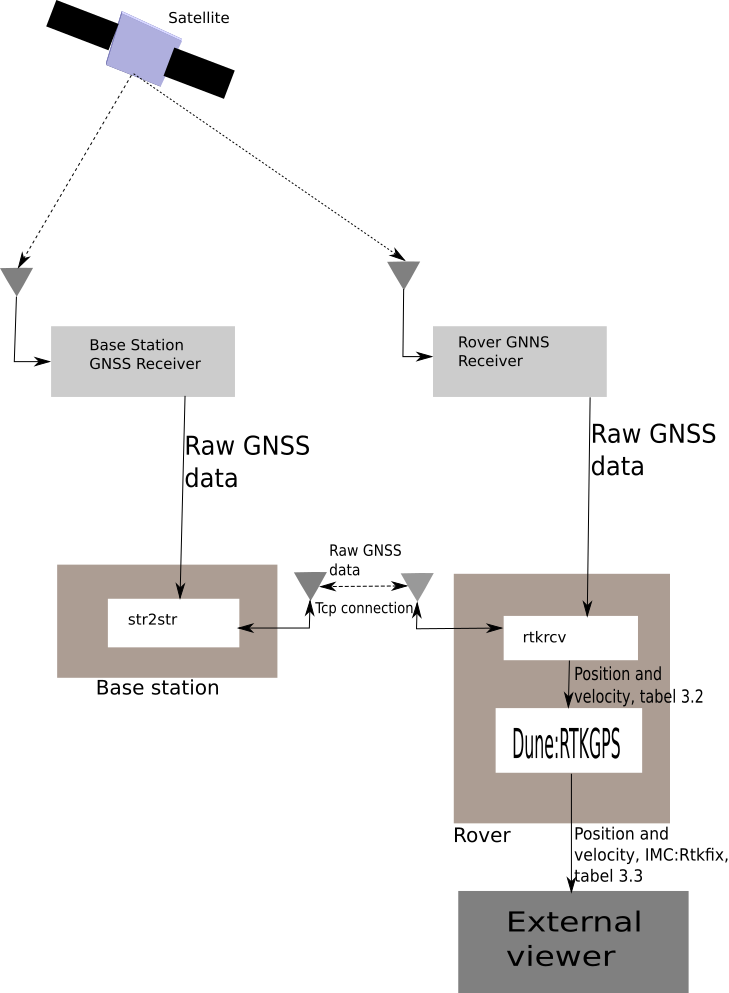
\includegraphics[width=0.7\textwidth]{figs/Rtklib_structure.png}
		\caption{The imu system and the true system}
		\label{figure:IMUSys}
\end{figure}
\subsubsection{rtkrcv}
Rtkrcv is the app program that calculate the position of the rovers antenna. Rtkrcv is configured with a moving baseline in order to get a fixed solution of the position estimate. Write about other design choices that affect the position output. 

Rtkrcv can be configured to have two output streams. The structure of the output stream is given the rtklib manual (Site it correctly). The solution body is given is table 
\begin{table}[!h]
\begin{center}
    \begin{tabular}{ | l | l |}
    \hline
    \textbf{Header} & \textbf{Content} \\ \hline
     1 Time & a1  \\ \hline
     2 Receiver Position & The rover receive antenna position \\ \hline
     3 Quality flag (Q) & The flag which indicates the solution quality.\\& 1:Fixed\\& 2:Float\\& 5:Single \\ \hline
     4 Number of valid satellites (ns) & The number of valid satellites for solution estimation. \\ \hline
     5 Standard deviation & The estimated standard deviation of the\\& solution assuming a priori error model and error parameters\\& by the positioning options \\ \hline
     6 Age of differential & The time difference between the observation data epochs\\& of the rover receiver and base station in second. \\ \hline
     7 Ratio factor & The ratio factor of "ratio-test" for standard integer\\& ambiguity validation strategy \\ \hline
    \end{tabular}
\end{center}
\caption{Table 1. }
\label{Tab1}
\end{table}
Rtkrcv uses the LAMDA search strategy for finding the ambiguity for the solution. 
\subsubsection{str2str}
Str2str is the app program that retrieve the ublox signal from the gps and sends over tcp to the rtkrcv app. The str2str is setup to either send RMTC 3 messages, or whatever is send in from the GPS. Since the str2str do not support to send ublox signal directly. How to write that the user should not specify the input format or the output format.
\section{Physical system}
This section outline the physical components in the x8 and the base station.
\subsection{Beaglebone}
The system runs on a Beaglebone. A beaglebone were prepared for mounting in a x8
\subsection{The GPS receiver}
Write about the Ublox LEA M8T gnss receiver. Also include that it support sending GPS and GLONASS data at the same time. Need to be configured. A receiver were prepare and mounted in the x8.
\cleardoublepage